\documentclass[a4paper,12pt]{article} % тип документа

%  Русский язык
\usepackage{multirow}
\usepackage{wrapfig}
\usepackage[T2A]{fontenc}			% кодировка
\usepackage[utf8]{inputenc}			% кодировка исходного текста
\usepackage[english,russian]{babel}	% локализация и переносы

\usepackage{indentfirst} %Красная строка
\usepackage[a4paper,top=1.3cm,bottom=2cm,left=1.5cm,right=1.5cm,marginparwidth=0.75cm]{geometry}
\usepackage[usenames]{color}
\usepackage{colortbl}
\usepackage{float}

\usepackage{graphicx}%картинки
\usepackage{textcomp}%Номер
\usepackage{wrapfig}%обтекание текстом теблиц и картинок
%гиперссылки
\usepackage{hyperref}
\usepackage[rgb]{xcolor}
\hypersetup{     %гипперсылки
 colorlinks=true, %false:ссылки в рамках
 urlcolor=blue   %на URL
 }
% Заметки
\usepackage{todonotes}
% Номера формул(необязятельна, см. по ситуации)
%\mathtoolsset{showonlyrefs=true} % Показывать номера только у тех формул, на которые есть \eqref{} в тексте.

% Математика
\usepackage{amsmath,amsfonts,amssymb,amsthm,mathtools} 
\usepackage{wasysym}

\usepackage{euscript} % Шрифт Евклид
\usepackage{mathrsfs} % Красивый матшрифт

\begin{document}

\begin{titlepage}
\begin{center}
    {\large МОСКОВСКИЙ ФИЗИКО-ТЕХНИЧЕСКИЙ ИНСТИТУТ (НАЦИОНАЛЬНЫЙ ИССЛЕДОВАТЕЛЬСКИЙ УНИВЕРСИТЕТ)}
\end{center}
\begin{center}
    {\largeФизтех-школа физики и исследований им. Ландау}
\end{center}

\vspace{3.5cm}

\begin{center}
    
\includegraphics[width=0.4\linewidth]{hv_full.png}
\end{center}
\vspace{0.1cm}
{\huge
\begin{center}
    {\bf Лабораторная работа 1.2.5}\\
    Исследование прецессии уравнавешанного гироскопа
\end{center}
}
\vspace{2cm}
\begin{flushright}
{\LARGE Авторы:\\ Петров Олег \\
\vspace{0.2cm}
Б02-202}
\end{flushright}
\vspace{3.5cm}
\begin{center}
    Долгопрудный 2022
\end{center}
\end{titlepage}

\section{Aннотация}
\textbf{Цель работы:} Исследование вынужденной регулярной прецессии гироскопа.
 Установление зависимости скорости вынужденной прецессии от величины момента сил трения, действующих на ось гироскопа.
 Определения скорости вращения ротора гироскопа и сравнение ее с расчитанной по скорости прецесии.\\

\textbf{Оборудование:} гироскоп,секундомер,набор грузов,отдельный ротор гироскопа,
 цилиндр известной массы, крутильный маятник,
 штангенциркуль, линейка.

\section{Теоретические сведения}
\subsection{Измерение частоты вращения ротора}

Гироскопом называется быстрo вращающиеся твердое тело для, для которого, момент
импульса относительно одной оси значительно больше момента импульса относительно других, например, вокруг оси $OZ$:
\begin{equation}
    \overrightarrow{L_z} \gg \overrightarrow{L_y}, \ \ \overrightarrow{L_x}
\end{equation}
Гироскоп уровновешен, если его центр масс неподвижен. А устойчивость вращения
 гироскопа связана с тем, что приращение момента импульса при действии внешних сил
 в течении короткого промежутка времени много меньше самого момента импульса и практически не
 иеняет его, то есть:
\begin{equation}
    |\Delta \overrightarrow{L}|=|\int \overrightarrow{M} dt |\ll |\overrightarrow{L} |
\end{equation}
Рассмотрим гироскоп вращающийся только относительно оси $OZ$ со скорость $\omega $.
Для того чтобы гироскоп начал совершать регуярную прецессию вокруг вертикальной оси $OY$ c угловой скорсть $\Omega$  
необходимо приложить к нему момент внешних сил $\overrightarrow{M}$ направленный вдоль оси $OX$. при этом если выполнено условие:
\begin{equation}
    \overrightarrow{L_{\Omega }} \ll \overrightarrow{L_{\omega}} 
\end{equation}
То момент имульса гироскопа относительно главной оси $\overrightarrow{L} $ практически не меняется со временем по модулю и связан
 с моментом приложенных сил $\overrightarrow{M}$ и скоростью прецессии $\Omega$ следующим соотношением:
\begin{equation}
    \overrightarrow{M}=\frac{d\overrightarrow{L}}{dt}=\overrightarrow{\Omega}\times \overrightarrow{L}
    \label{MLQ}
\end{equation}
Для изучения регулярной прецесии уравновешанного гироскопа подвесим к нему дополнительные грузы.
 Это смещает общий центр масс и создает момент силы тяжести,
 вызывающий прецессию. Тогда скорость вращения ротора гироскопа равна:
\begin{equation}
    \omega=\frac{L}{I_{z}}=\frac{M}{I_{z}\Omega},\ \ \ \text{где} \ M=mgl
\end{equation}

\subsection{Измерение момента инерции ротора}

Момент инерции ротора измеряем по периоду крутильных колебаний на жесткой проволке.
Чтобы исключить модуль кручения проволки $f$, подвешиваем цилиндр правильной формы с известным моментом инерции $I_{ц}$

\begin{equation}
    T=2\pi\sqrt{\frac{I}{f}},\ \  \ \ \ \  I=I_\text{ц}\frac{T^2}{T^2_\text{ц}}
    \label{T}
\end{equation}

\subsection{Измерени момента сил трения}

Так как силы трения имеют составляющую, не лежащую в плоскости осей вращения,
они меняют момент импульса и по направлению, и по величине. Для ротора гироскопа
действие сил трение скомпенсировано электромотором, для осей карданова подвеса компенсации
нет. В результате чего ось гироскопа будет опускатья в направлении действия груза.
Момент сил трения $M_\text{тр}$ может быть вычислен по формуле:
\begin{equation}
    M_\text{тр}=\frac{\Delta\alpha}{t}L
\end{equation}

%\section*{Экспериментальная установка}
\section{Результаты эксперимента и обраюотка данных}
\subsection{Измерение момента импульса ротора}
Отклоним рычаг на 5-6 градусов в верх и подвесим к нему груз. Результаты измерении числа оборотов,
времени движения и всего осатльного заносим в  табличу один \ref{table1}. Установим параметры системы
и систематические погрешности:$$l=121\pm 1 \ \text{мм}, \ \ g=9.815 \pm 0.005 \ \text{м}c^{-2}$$,
$$\Delta m=1 \ \text{г},\ \ \Delta T = 0.1 \ c  $$
Расчет угла, на который опускается вертикальная ось, заносим в таблицу и производим по формуле : 
$$\Delta\alpha=\frac{\Delta h}{l} \cdot \frac{180}{\pi}  $$

\begin{table}[!h]
\begin{center}
\label{table1}
\begin{tabular}{|l|r|r|r|r|r|r|r|} \hline
        №  & $m,гр$ & $t,c$ & $N$ & $\Delta h, \text{мм}$ & $\Delta \alpha,\circ  $ & $T,c$ & $\Delta\alpha /T, \circ \cdot c^{-1} $ \\ \hline
        1  &  61  &  168.4 &  1 &  5 &  2.37 &  168.4 &  0.014\\ \hline
        2  &  61  &  170.9 &  1 &  5 &  2.37 &  170.9 &  0.014\\ \hline
        3  &  93  &  221.3 &  2 &  8 &  3.79 &  110.7 &  0.017\\ \hline
        4  &  93  &  222.6 &  2 &  7 &  3.32 &  111.3 &  0.015\\ \hline
        5  &  93  &  221.6 &  2 &  8 &  3.79 &  110.8 &  0.017\\ \hline
        6  &  142 &  216.6 &  3 &  9 &  4.26 &  72.2  &  0.020\\ \hline
        7  &  142 &  215   &  3 &  8 &  3.79 &  71.7  &  0.018\\ \hline
        8  &  142 &  215.8 &  3 &  9 &  4.26 &  71.9  &  0.020\\ \hline
        9  &  214 &  143   &  3 &  4 &  1.90 &  47.7  &  0.013\\ \hline
        10 &  214 &  143   &  3 &  3 &  1.42 &  47.7  &  0.010\\ \hline
        1 &  335 &  122.2 &  4 &  5 &  2.37 &  30.6  &  0.019\\ \hline
        12 &  335 &  123.7 &  4 &  5 &  2.37 &  30.9  &  0.019\\ \hline
        13 &  335 &  125.1 &  4 &  4 &  1.90 &  31.3  &  0.015\\ \hline
        14 &  335 &  122.7 &  4 &  5 &  2.37 &  30.7  &  0.019\\ \hline
\end{tabular}
\caption{Все измерения величин}
\end{center}
\end{table}
 
Усредняем значения периода для выборки с одинаковой массой и заносим результаты в таблицу \ref{table2}.
Погрешность измерения периода оцениваем по формуле:
$$\sigma^T_\text{случ}=\sqrt{\sum_{i} (T_{i}-\langle T \rangle)^2 /N }, \ \ \ \sigma^T_\text{сист}=\Delta T/ N$$,
$$\sigma_{T}=\sqrt{\sigma^2_\text{случ}+\sigma^2_\text{сист}}$$
Тогда скорость прецесии и ее погрешность вычисляем по формуле по формуле:
$$\Omega=\frac{2\pi}{T}, \ \ \sigma_{\Omega}=\frac{\Omega}{T}\cdot \sigma_{T}$$
И аналогично для вычисления момента сил тяжести имеем:
$$M=mgl, \ \ \sigma_{M}=M\sqrt{\left(\dfrac{\Delta m}{m}\right)^2+\left(\dfrac{\Delta l}{l}\right)^2}$$
Средние относительные погрешности измерений $\Omega$ и $M$, таким образом получаются $\varepsilon_{\Omega}=0.3\% $ и $\varepsilon_{M}=1.3 \%$.

\begin{table}[h!]
\begin{center}
\label{table2}
\begin{tabular}{|l|r|r|r|r|r|r|r|r|}\hline
        № & $m,гр$ &$T,c$&$\sigma_{T}$,c&$\Omega, 10^-2$c &$\sigma_{\Omega}, 10^-2$ c &$M, 10^-2$Нм&$\sigma_{M}, 10^-2$ Нм \\ \hline
        1 &  61  &  169.7 &  1.6 &  3.70    &  0.03    &  7.2      &  0.1\\ \hline
        2 &  93  &  110.9 &  0.1 &  5.66    &  0.01    &  11.0     &  0.1\\ \hline
        3 &  142 &  71.9  &  0.1 &  8.73    &  0.01    &  16.9     &  0.2\\ \hline
        4 &  214 &  47.7  &  0.1 &  13.18   &  0.03    &  25.4     &  0.2\\ \hline
        5 &  335 &  30.9  &  0.1 &  20.36   &  0.05    &  39.8     &  0.3\\ \hline
\end{tabular}
\caption{Все измерения величин}
\end{center}
\end{table}

Построим график зависимости $M(\Omega)$ пользуясь методом наименьших квадратов(МНК):
\begin{figure}[!h]
    \begin{center}
        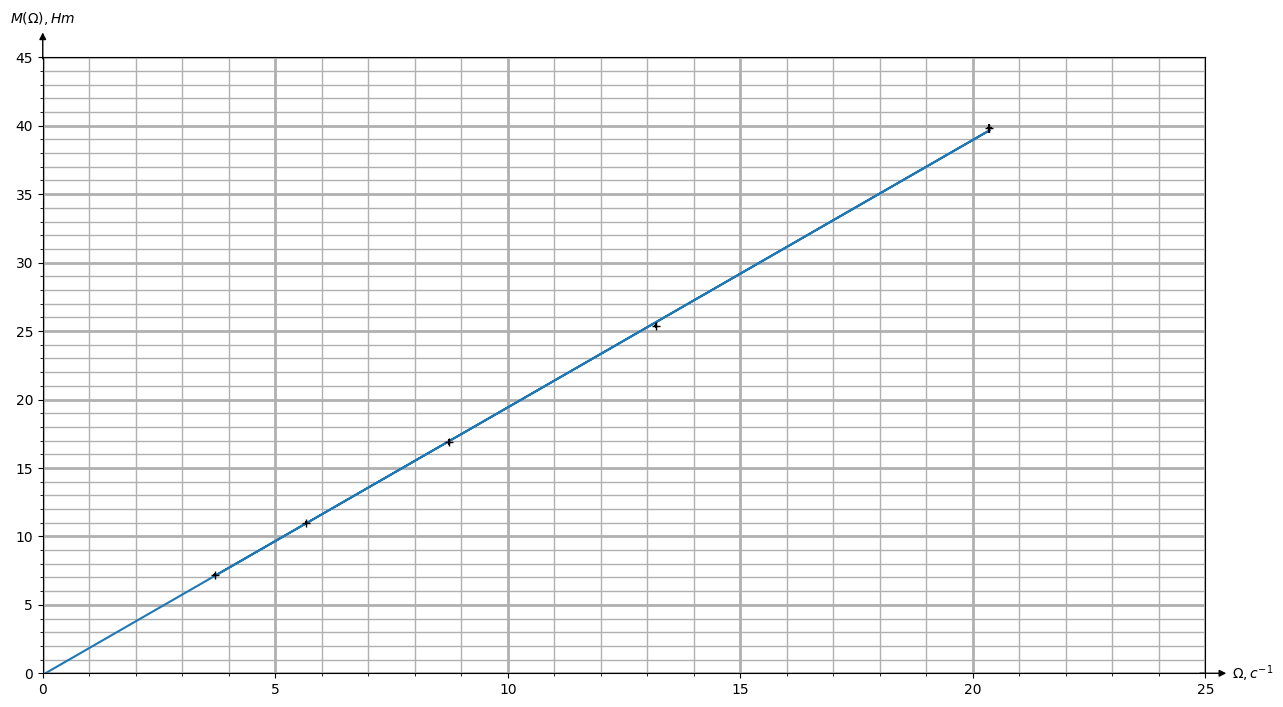
\includegraphics[width=1\textwidth]{graphic}
        \caption{График зависимости $M$ от $\Omega$}
        \label{graphic1}
    \end{center}
\end{figure}

Воспользовавшись формулой \eqref{MLQ} получим, что коэффицент наклона графика $k=M/ \Omega=L$.
Пользуясь формулами МНК найдем коэффицент:
$$L=\dfrac{\langle M\Omega \rangle-\langle \Omega \rangle \langle M\rangle}{\langle \Omega^2\rangle - \langle \Omega\rangle^2} = 1.95 \ \text{$\dfrac{\text{кг}\ \text{м}^2}{\text{c}}$}$$
Для оценки погрешноси L имеем:\\
$$\sigma_L^\text{случ}=\frac{1}{\sqrt{3}}\sqrt{\frac{\langle M^2 \rangle - \langle M \rangle^2}{\langle \Omega^2 \rangle - \langle \Omega \rangle^2} - k^2 }
 = 0.03\ \text{$\dfrac{\text{кг}\ \text{м}^2}{\text{c}}$}, \ \ \ 
\sigma_L^\text{сист}=L\sqrt{\left \langle \frac{\sigma_{M}}{M}\right \rangle ^2
 + \left \langle \frac{\sigma_{\Omega}}{\Omega}\right \rangle^2}
  = 0.02 \ \text{$\dfrac{\text{кг}\ \text{м}^2}{\text{c}}$}$$
%можно заметить, что $\sigma_\text{случ} \gg \sigma^2_\text{сист}/2\sigma_\text{случ}$,
%это означет, что в первом приближении $\sigma_\text{случ}\thickapprox \sigma_L$,
%что и поддтверждает расчет ниже:
$$\sigma_L=\sqrt{\sigma_\text{сист}^2+\sigma_\text{случ}^2}=0.03 \ \text{$\dfrac{\text{кг}\ \text{м}^2}{\text{c}}$}, \ \ \ \varepsilon_{L}= 1.5 \% $$
Таким образом получаем итоговое значение момента импульса $L=1.95 \pm \ 0.03 \  кг\text{м}^2\text{c}^{-1}$.

\subsection{Измерение момента инерции ротора}
Измерим момент инерции ротора гироскопа относительно оси симметрии $I$.
Для этого подвесим ротор и цилиндр к концу стальной нити и возбудим крутильные колебания.
Время для $N=20$ колебний ротора и цилиндра заносим в таблицу \ref{}. 
Расчеты будем проводить по формулам \eqref{T}. Параметры системы:
$$m_{\text{ц}}=1616.9\ \text{гр}, \ \ \ R_{\text{ц}}=38.5\ \text{мм}$$,
$$ \Delta T=1\ \text{c},\ \ \Delta m_{\text{ц}}=0.1\ \text{гр}, \ \ \Delta R_{\text{ц}}=0.1\ \text{мм}$$

\begin{table}[!h]
    \begin{center}
        \label{table3}
        \begin{tabular}{|l|r|r|r|r|} \hline
            № & $N=20,T$,c & $N=20$,$T_{\text{ц}}$,c & $T$,c & $T_{\text{ц}}$,c \\ \hline
             1 &  63.6 &  78.8 &  3.18 &  3.94 \\ \hline
             2 &  64.2 &  78.7 &  3.21 &  3.935\\ \hline
             3 &  66.6 &  81   &  3.33 &  4.05 \\ \hline
            \end{tabular}
        \caption{Результаты измеренй периода}
    \end{center}
\end{table}

За итоговое значение периода принимаем усредненный по выборке $\langle T \rangle $,
погрешность измерения периода оцениваем как:
$$\sigma^T_\text{случ}=\sqrt{\sum_{i} (T_{i}-\langle T \rangle)^2 /N }, \ \ \ \sigma^T_\text{сист}=\Delta T/ N, \ \ \ 
\sigma_{T}=\sqrt{\sigma^2_\text{случ}+\sigma^2_\text{сист}}$$
Для $T$ и $T_{\text{ц}}$ получаем конкретные значения периода и погрешностей:
$$T_{\text{ц}}=3.975 \ \text{c}, \ \ \ \sigma_{T_{\text{ц}}}=0.006\ \text{c} \ \ \ \varepsilon_{T_{\text{ц}}}=0.07 \% $$
$$T=3.240\ \text{c},\ \ \ \sigma_{T}=0.006\ \text{c} \ \ \ \varepsilon_{T}=0.13\% $$
Тогда для момента инерции цилиндра $I_{\text{ц}}$ и его погрешности имеем:
$$I_{\text{ц}}=m_{\text{ц}}\cdot R^2_{\text{ц}}= 1.198 \ 10^{-3} \ \text{кг}\cdot\text{м}^2, \ \ \ 
\sigma_{I_{\text{ц}}}=I_{\text{ц}}
\sqrt{\left(\frac{\Delta m_{\text{ц}}}{m_{\text{ц}}}\right)^2
+\left(\frac{2 \Delta R_{\text{ц}}}{R_{\text{ц}}}\right)^2}\approx 0.006 \ 10^{-3}\text{кг}\cdot\text{м}^2, \ \ \
\varepsilon_{I_{\text{ц}}}=0.5 \% $$
Тогда для итогового значения момента импульса $I$ и его погрешности имеем:
$$I=I_{\text{ц}}\cdot\frac{T^2}{T^2_{\text{ц}}}=0.796 \ 10^{-3}\text{кг}\cdot\text{м}^2$$
C учетом $\varepsilon_{I_{\text{ц}} \gg  \varepsilon_{T}, \ \ \varepsilon_{T_{\text{ц}}}$ получаем,что
$\varepsilon_{I_{\text{ц}} \approx \varepsilon_{I} = 0.5 \% $  и итого для погрешности измерения имееем:
$$\sigma_{I}=I\sqrt{\left(\varepsilon_{I_{\text{ц}}}\right)^2
+\left(2\varepsilon_{T}\right)^2 
+\left(2\varepsilon_{T_{\text{ц}}}\right)^2}\approx \varepsilon_{I_{\text{ц}}}\cdot I = 0.004 \ 10^{-3} \text{кг} \cdot \text{м}^2$$

То есть получаем тоговое значение для момента инерции:$$I=0.796 \pm 0.004 \ 10^{-3}\text{кг} \cdot \text{м}^2, \varepsilon_{I} = 0.5 \% $$

\subsection{Измерение частоты вращения ротора}
Зная момент импульса и момент инерции ротора, легко вычисляем частоту его вращения и погрешность
измерения по формулам:
$$f=\frac{L}{2\pi I}=390 \ \text{Гц}, \ \ \ \sigma_{f}=f\sqrt{\varepsilon_{I}^2+\varepsilon_{L}^2}\approx \varepsilon_{L}\cdot f = 6 \ \text{Гц},
 \ \ \ \varepsilon_{f}=1.6\% $$
Итого для частоты имеем: $f=390\pm 6 \ \text{Гц}$
Также при измерении частоты с помощью осциллографа и цифрового частотометра было получено значение:
$$f_{осц}=390 \pm 1 \ \text{Гц}$$

\subsection{Измерени момента сил трения}
Во время эксперимента трение в вертикальной оси не было скомпенсированно.
Поэтому ось гироскопа незначительно опускалась. Для оценки сил трения
будем измерять высоту на которую вертикально опустился груз $\Delta h$ за время $t$ и 
рассчитывать с помощью него угол $\alpha = \Delta h / l$. Данные заносим в таблицу:

\begin{table}[!h]
    \begin{center}
        \label{table4}
            \begin{tabular}{|l|l|l|l|l|}\hline
            №  & $t,c$ & $\Delta h,\text{мм}$&$\Delta \alpha,\circ$& $M_{\text{тр}},$ Нм\\ \hline
            1  & 168.4 & 5 & 2.37 & 4.9 \\ \hline
            2  & 170.9 & 5 & 2.38 & 4.7 \\ \hline
            3  & 221.3 & 8 & 3.79 & 5.8  \\ \hline
            4  & 222.6 & 7 & 3.31 & 5.1 \\ \hline
            5  & 221.6 & 8 & 3.79 & 5.8 \\ \hline 
            6  & 216.6 & 9 & 4.27  & 6.7 \\ \hline
            7  & 215   & 8 & 3.79 & 6.0  \\ \hline
            8  & 215.8 & 9 & 4.26  & 6.7 \\ \hline
            9  & 143   & 4 & 1.89 & 4.5 \\ \hline
            10 & 143   & 3 & 1.42 & 3.4 \\ \hline
            11 & 122.2 & 5 & 2.37 & 6.6 \\ \hline
            12 & 123.7 & 5 & 2.37 & 6.5 \\ \hline
            13 & 125.1 & 4 & 1.89 & 5.2 \\ \hline
            14 & 122.7 & 5 & 2.37 & 6.6 \\ \hline
            \end{tabular}
        \caption{Измерение момента сил трения}
    \end{center}
\end{table}

Расчет значения в каждом измерении делаем по формуле:
$$M_\text{тр}=\frac{\Delta\alpha}{t}L=\frac{L}{2\pi t}\cdot \frac{\Delta h}{l}$$
За итоговое значение $M_\text{тр}$ принимаем усредненное по всей выборке.
В силу большой несовершенности методики измерений $\Delta h, \alpha$ существенную ошибку 
дает систематическая погрешность измерения $\sigma_{\Delta h}=0.5$ мм со средней
относительной погрешностью $\varepsilon_{\Delta h}=9 \%$. Все остальные факторы имеют
значительно меньшую относительную погрешность, а потому их можно отбросить
и считать, что
$$\varepsilon_{M_{\text{тр}}}=\varepsilon_{\Delta h}=9 \%, \ \ \ \sigma_{M_{\text{тр}}}=\varepsilon_{M_{\text{тр}}}\cdot M_{\text{тр}}= 0.5 \ \text{Hм}$$
Итого получаем значением момента силы трения: $$M_{\text{тр}}= 5.6 \pm 0.5 \ \text{Hм}$$

\section{Выводы}
Получены результаты хорошо согласующие с теоретическими предсказаниями. 
Поддтверждена линйная зависимость между моментом сил и скоростью прецессии.
Получено значение частоты $f=390 \pm 6 \ \text{Гц}$ хорошо согласующее с измеренным $f_{осц}=390 \pm 1 \ \text{Гц}$. 
\end{document}